
% Template for Elsevier CRC journal article
% version 1.1 dated 16 March 2010

% This file (c) 2010 Elsevier Ltd.  Modifications may be freely made,
% provided the edited file is saved under a different name

% This file contains modifications for Procedia Computer Science
% but may easily be adapted to other journals

% Changes since version 1.0
% - elsarticle class option changed from 1p to 3p (to better reflect CRC layout)

%-----------------------------------------------------------------------------------

%% This template uses the elsarticle.cls document class and the extension package ecrc.sty
%% For full documentation on usage of elsarticle.cls, consult the documentation "elsdoc.pdf"
%% Further resources available at http://www.elsevier.com/latex

%-----------------------------------------------------------------------------------

%%%%%%%%%%%%%%%%%%%%%%%%%%%%%%%%%%%%%%%%%%%%%%
%%%%%%%%%%%%%%%%%%%%%%%%%%%%%%%%%%%%%%%%%%%%%%
%%                                          %%
%% Important note on usage                  %%
%% -----------------------                  %%
%% This file must be compiled with PDFLaTeX %%
%% Using standard LaTeX will not work!      %%
%%                                          %%
%%%%%%%%%%%%%%%%%%%%%%%%%%%%%%%%%%%%%%%%%%%%%%
%%%%%%%%%%%%%%%%%%%%%%%%%%%%%%%%%%%%%%%%%%%%%%

%% The '3p' and 'times' class options of elsarticle are used for Elsevier CRC
\documentclass[3p,times]{elsarticle}

%% The `ecrc' package must be called to make the CRC functionality available
\usepackage{ecrc}

%% The ecrc package defines commands needed for running heads and logos.
%% For running heads, you can set the journal name, the volume, the starting page and the authors

%% set the volume if you know. Otherwise `00'
\volume{00}

%% set the starting page if not 1
\firstpage{1}

%% Give the name of the journal
\journalname{NUCLEAR INSTRUMENTS AND METHODS
IN PHYSICS RESEARCH}

%% Give the author list to appear in the running head
%% Example \runauth{C.V. Radhakrishnan et al.}
\runauth{D. E. Holland et al.}

%% The choice of journal logo is determined by the \jid and \jnltitlelogo commands.
%% A user-supplied logo with the name <\jid>logo.pdf will be inserted if present.
%% e.g. if \jid{yspmi} the system will look for a file yspmilogo.pdf
%% Otherwise the content of \jnltitlelogo will be set between horizontal lines as a default logo

%% Give the abbreviation of the Journal.
\jid{NIM:A}

%% Give a short journal name for the dummy logo (if needed)
\jnltitlelogo{NIM:A}

%% Hereafter the template follows `elsarticle'.
%% For more details see the existing template files elsarticle-template-harv.tex and elsarticle-template-num.tex.

%% Elsevier CRC generally uses a numbered reference style
%% For this, the conventions of elsarticle-template-num.tex should be followed (included below)
%% If using BibTeX, use the style file elsarticle-num.bst

%% End of ecrc-specific commands
%%%%%%%%%%%%%%%%%%%%%%%%%%%%%%%%%%%%%%%%%%%%%%%%%%%%%%%%%%%%%%%%%%%%%%%%%%

%% The amssymb package provides various useful mathematical symbols
\usepackage{amssymb}
%% The amsthm package provides extended theorem environments
\usepackage{amsthm}
\usepackage{amsmath}

%% The lineno packages adds line numbers. Start line numbering with
%% \begin{linenumbers}, end it with \end{linenumbers}. Or switch it on
%% for the whole article with \linenumbers after \end{frontmatter}.
%% \usepackage{lineno}

%% natbib.sty is loaded by default. However, natbib options can be
%% provided with \biboptions{...} command. Following options are
%% valid:

%%   round  -  round parentheses are used (default)
%%   square -  square brackets are used   [option]
%%   curly  -  curly braces are used      {option}
%%   angle  -  angle brackets are used    <option>
%%   semicolon  -  multiple citations separated by semi-colon
%%   colon  - same as semicolon, an earlier confusion
%%   comma  -  separated by comma
%%   numbers-  selects numerical citations
%%   super  -  numerical citations as superscripts
%%   sort   -  sorts multiple citations according to order in ref. list
%%   sort&compress   -  like sort, but also compresses numerical citations
%%   compress - compresses without sorting
%%
%% \biboptions{comma,round}

% \biboptions{}

% if you have landscape tables
\usepackage[figuresright]{rotating}

% put your own definitions here:
%   \newcommand{\cZ}{\cal{Z}}
%   \newtheorem{def}{Definition}[section]
%   ...

% add words to TeX's hyphenation exception list
%\hyphenation{author another created financial paper re-commend-ed Post-Script}

% declarations for front matter

\begin{document}

\begin{frontmatter}

%% Title, authors and addresses

%% use the tnoteref command within \title for footnotes;
%% use the tnotetext command for the associated footnote;
%% use the fnref command within \author or \address for footnotes;
%% use the fntext command for the associated footnote;
%% use the corref command within \author for corresponding author footnotes;
%% use the cortext command for the associated footnote;
%% use the ead command for the email address,
%% and the form \ead[url] for the home page:
%%
%% \title{Title\tnoteref{label1}}
%% \tnotetext[label1]{}
%% \author{Name\corref{cor1}\fnref{label2}}
%% \ead{email address}
%% \ead[url]{home page}
%% \fntext[label2]{}
%% \cortext[cor1]{}
%% \address{Address\fnref{label3}}
%% \fntext[label3]{}

\dochead{}
%% Use \dochead if there is an article header, e.g. \dochead{Short communication}

\title{Rotating Scatter Mask Optimization for Gamma Source Location Identification}

%% use optional labels to link authors explicitly to addresses:
%% \author[label1,label2]{<author name>}
%% \address[label1]{<address>}
%% \address[label2]{<address>}

\author[d1]{Darren E. Holland}

\address[d1]{dholland@cedarville.edu\\
  Department of Mechanical Engineering\\
	Cedarville University \\
	Cedarville, OH 45502 USA\\}

\begin{abstract}
Rotating scattering masks have shown promise as a cheap, lightweight method for identifying the direction of a gamma emitting source.
However, further examination of the current rotating scattering mask design shows that the identification could be improved by changing the geometry.  
Three methods are introduced to generate the mask geometry accompanied by the resulting detector response matrix analysis.  
The results demonstrate superior identification characteristics than the current design.  
Further possible design enhancements are discussed.
\end{abstract}

\begin{keyword}
%% keywords here, in the form: keyword \sep keyword
RSM \sep geometry optimization \sep Hadamard \sep source direction
%% MSC codes here, in the form: \MSC code \sep code
%% or \MSC[2008] code \sep code (2000 is the default)

\end{keyword}

\end{frontmatter}

%%
%% Start line numbering here if you want
%%
% \linenumbers

%% main text
\section{Introduction}
\label{intro}
Identifying a gamma source's location is important in a variety of situations such as providing security, treaty compliance, and locating orphan sources.  
% We need to add a couple sentences with a couple references about alternative approaches.  A quick detail of their performance characteristics would also be beneficial.

A novel alternative approach utilizes a mask placed over a position-insensitive detector \cite{FitzGerald2015}.  
The system records energy spectra as a function of the geometrically varying mask, which is accomplished through a constant rotation of the mask at a set rate. 
The spectra obtained depend on the source position and can be used to identify the source direction.  

\section{Background}
The rotating scatter mask (RSM) concept offers many benefits over other gamma source position identification detectors.  
Specifically, it "provides a nearly 4$\pi$ field-of-view, operates for a broad range of gamma energies, and has a relatively simple design \cite{Logan2017}." 
This system uses a spherical reference system, where $\theta$ is the azimuthal and $\phi$ the polar angle.  
The mask works by attenuating and scattering the incoming particles in order to produce unique detector response curves (DRCs) \cite{Logan2017}.  
To obtain the measurements for the position identification, the mask starts at an initial $\theta$ and $\phi$ position.
It then rotates in $\theta$ around the detector with the signal recorded at each discrete $\theta$ position.  
The measured DRC is generated by summing the counts over a desired full energy peak for each $\theta$ position in one complete mask rotation.  
Comparing this curve with each possible DRC, which are known through experimentation or simulation, using a mean square error, least squares, or maximum likelihood estimate approach provides an identified initial source location.

FitzGerald introduced the RSM shown in Fig.~\ref{fig:RSM} that has a 14 inch diameter and surrounds a 3 x 3 inch cylindrical NaI scintillating detector \cite{FitzGerald2015}. 
His original MCNP model contained 31 elements or one element every $11.6^\circ$.  
In order to increase the accuracy of the geometric representations,  the angular resolution of the model was later increased to every degree.  

\begin{figure}[ht!]
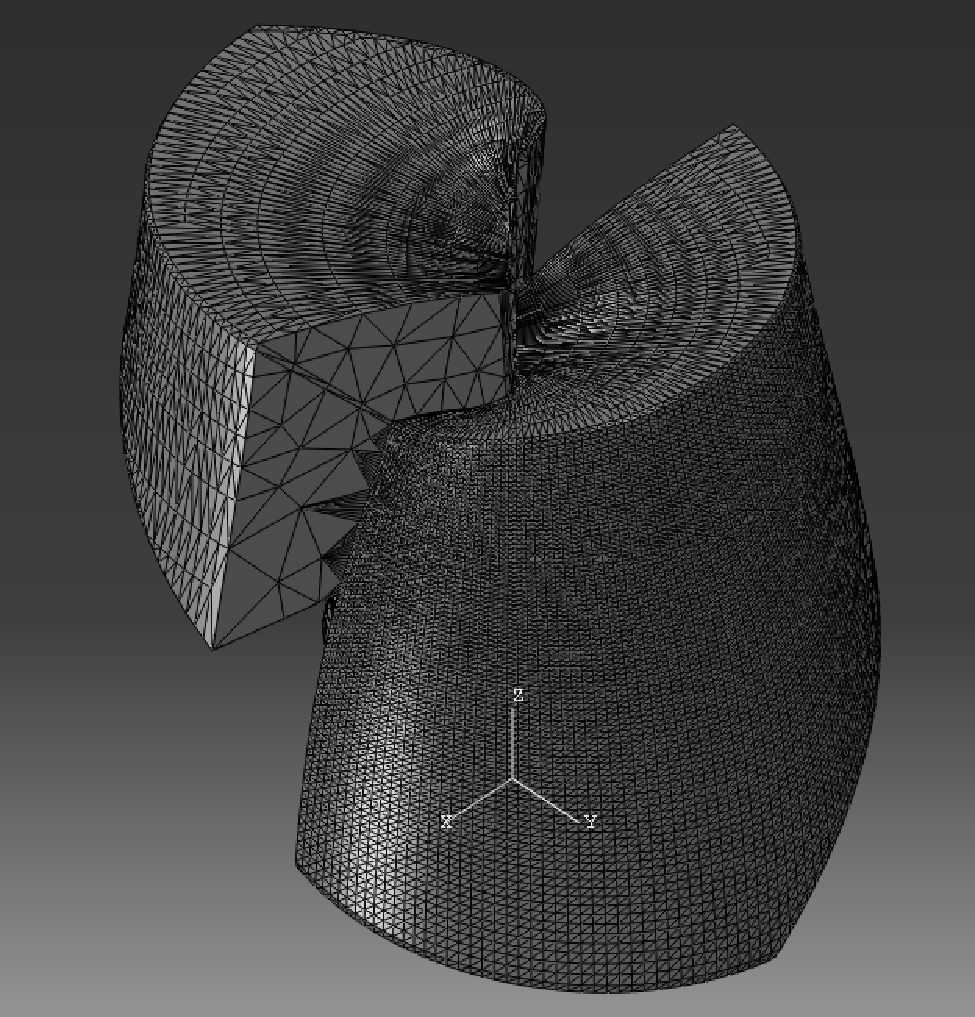
\includegraphics[width={3.0in}]{../figs/P2AtIso.pdf}
\centering
\caption{An isometric view of the unstructured mesh used to model the RSM in MCNP}
\label{fig:RSM}
\end{figure}

FitzGerald's design methodology assumes that the detector response is related to the mask geometry.  
Without this assumption, intentional mask design degenerates into random trial and error.
In addition, he proposed three desirable characteristics for the RSM system.  
First, for any given initial source position, there is a unique response curve generated as the mask rotates 360$^\circ$.  
This condition is necessary as a non-unique response would make at least two initial source position DRCs indistinguishable and unique identification impossible.
The second characteristic requires the mask's average thickness over a 360$^\circ$ rotation to be a constant value for all $\phi$s.  
This criteria prevents higher or lower average responses for different $\phi$ positions. 
This is not necessary to ensure the uniqueness of the DRC, however DRCs with widely varying average thicknesses may have a lower average count, which makes them more susceptible to measurement noise and increases the time required to obtain an accurate measured response.
The final characteristic is for the solid angle from the detector centroid to be equal for all cells.  
This constraint provides the same spacial resolution in both azimuthal and polar directions.
Not explicitly mentioned by FitzGerald is an assumption that the geometry should be continuous, thereby allowing the DRCs to be discretized as desired.

To improve upon the Fitzgerald design, methods were borrowed from the design of encoding masks is in the fields of spectrometry and imaging \cite{Sloane76, Finger85, Hanley00, DeVerse00}, where similar work was done to produce a rotating encoding mask \cite{Bellamy97}.
Fateley et al.\cite{Fateley00} introduced the use of frequency information to identify spatial position information.
% Each of which methods? The preceeding and following sentences seem a bit disjointed, but I think the goal is to say that Fateley introduced the idea of using frequency information for REM design which was based on Hadamard matrices. I didn't want to reword in case that reading was incorrect.  
Each of these methods is based on using a Hadamard matrix for the mask design.

\section{Basic Model Setup}
Originally, both the analysis of FitzGerald's RSM and the new designs were to be discretized into 10$^\circ$ increments in $\theta$ and 5$^\circ$ in $\phi$.  
However, due to requirements for the Hadamard method, (which is discussed later) 
the proposed designs are broken into 32 discrete angles in $\theta$ resulting in $\Delta\theta=11.25^\circ$ and $\Delta\phi=5.625^\circ$ for 30 angles in $\phi$.

The RSM design is to be optimized for a $^{137}$Cs point source located at 36 inches from the center of the detector, mimicking Logan et. al's setup \cite{Logan2017}.  
To simulate the relative source rotation in MCNP, the mask is stationary, while the source is rotated in spherical coordinates every degree for $\theta$ from 0 to $348.75^\circ$ and for each $\phi$ from 5.625$^\circ$ to $168.75^\circ$.  
The modeled NaI detector includes a 1/8 inch 2024 Aluminum alloy sleeve on which the acrylic RSM is placed. 
The maximum diameter of the RSM depends on the methodology, but the maximum mask thickness is a constant 7.87 inches (20 cm).  
A sphere of air surrounds the source and detector.  
To increase the solution convergence rate, particles were emitted within a $27.26^\circ$ half angle cone extending from the source to the detector's center.  
This variance reduction technique assumes that the effect of the few particles that 
scatter in the air outside of the cone, though the mask, and into the detector will not contribute to the full energy peak and not affect the simulated DRCs.   
In addition, a 0.095 inch air gap between the mask and aluminum sleeve constrains the mask geometry from impinging on the sleeve and provides a space for grease to be applied between the moving parts.
Finally, due to manufacturing constraints, each mask angle must have a non-zero thickness.

\section{Design Assumptions}
Monte Carlo N-Particle (MCNP) is one method used to simulate energy spectrum.  
Logan et al.\cite{Logan2017} showed statistical agreement between experimental and simulated DRCs.  
Thus, this work will use simulated DRCs to evaluate the RSM performance.  
Instead of the full energy peak (FEP), the DRC is formed by adding all counts above 200keV.  
This value was chosen as Logan et al. noted discrepancies due to scatter in the enclosing environment for counts below approximately 200keV.

Herein, it is assumed that the geometry is related to the DRC.  
Qualitative studies of this correlation showed that in general, this assumption is valid with two qualifications.  
First, a discontinuous geometry results in a continuous DRC.  
To understand the next qualification, define a cell to be a rectangular prism with a given thickness extending from the centroid of the detector (outside of the Aluminum sleeve) in a given direction.
Since the cells do not have impenetrable walls, particles from one source position enter cells pointed at other positions.  
In fact, this phenomena is one of the desirable characteristics of FitzGerald's design as an increase in scattered particles can increase the total number of counts seen by the detector.  
Unfortunately, there is a corresponding limit to the spacial resolution.  
When the solid angle for a cell becomes too small, it is possible that the source does not resemble a point source, but a distributed source (which spans multiple cells) as neighboring cells also include a strong response.

As the desire is to obtain a unique set of DRCs, which can be placed in a detector response matrix (DRM), the primary criterion for the design will be choosing a design with the most unique DRM.  
To achieve this goal, the requirements for maintaining a constant spacial resolution in both spherical directions and requiring a continuous geometry are relaxed.  
However, to obtain a more constant response level a constant average thickness is maintained.  

To assess the design optimality, three criteria are proposed.  
The first is the modal assurance criterion (MAC).  This normalized number indicates the similarity between two vectors\cite{Allemang03}.  
A MAC value of 0 indicates the two vectors are orthogonal, while a value of 1 indicates that they are identical.  
For this application, it is desirable that the curve generated at each initial source position be orthogonal aka unique to the others.  
Let this curve be denoted $\mathbf{DRC}_{i,j}$ where $i=0,1,...,n$ is the initial $\theta$ and $j=0,1,...,m$ is the initial $\phi$ index (aka discrete position) relative to a reference location on the mask.  
Since the mask rotates, the $i^{th}$ DRC will be identical to the $k^{th}$ curve shifted by $k-i$ indices.  
A negative number corresponds to a shift to the left and a positive number a shift to the right.  
This property greatly impacts the mask design as any periodic vector with respect to $\theta$ will then result in duplicate $i$ and $k$ DRCs.  
The duplication fails to meet the design's uniqueness requirement.

Logan's work established a connection between the measured and the simulated DRCs.  Thus, assuming the measured response can be represented by the simulated spectrum, it is possible to analyze the uniqueness of the design by comparing each DRC with every other possible DRC to find the worst and average performance.  
Equation~\ref{eq:mac} defines the MAC number as

\begin{equation}
MAC_{i,j,k,l}=\frac{\left(\mathbf{u}_{i,j}^T\mathbf{v}_{k,l}\right)^2}{\left(\mathbf{u}_{i,j}^T\mathbf{u}_{i,j}\right)\left(\mathbf{v}_{k,l}^T\mathbf{v}_{k,l}\right)},
\label{eq:mac}
\end{equation}
where $\mathbf{u}_{i,j}$ and $\mathbf{v}_{k,l}$ are the DRCs for the respective initial positions $\left(\theta=i\Delta\theta,\phi=j\Delta\phi\right)$ and
$\left(\theta=k\Delta\theta,\phi=l\Delta\phi\right)$.

Considering the vector shifts, the maximum MAC number, which corresponds to the most similar pair of DRCs, and the average MAC number are given in Eqns.~\ref{eq:maxmac} and \ref{eq:avgmac} respectively.

\begin{equation}
M=max_{i,j,k,l}\left(MAC_{i,j,k,l}\right),
\label{eq:maxmac}
\end{equation}

where $i\neq k$ and $j\neq l$.

\begin{equation}
A=\frac{1}{b}\sum_{i,j,k,l}\left(MAC_{i,j,k,l}\right),
\label{eq:avgmac}
\end{equation}

where $i\neq k$, $j\neq l$, and $b$ is the total number of combinations given by $b=\left(\overset{m}{_2}\right)+(n-1)\left(\overset{m+1}{_2}\right)$.  
Note that $\left(\overset{m}{_2}\right)$ is the total number of combinations without $\theta$ shifts (aka $\theta=0$), $n-1$ is the total number of $\theta$ shifts possible, and $\left(\overset{m+1}{_2}\right)$ is the number of combinations for DRCs shifted one $\theta$ position.  
For the $n=32$ and $m=30$ mask design, $b=14850$.  
An examination of Eqn.~\ref{eq:maxmac} shows that a bias in vectors $u$ and $v$ will result in a non-zero $M$ value.  
Thus, the DRCs are normalized such that each one is zero mean over $\theta$.  
These normalized values form the reduced DRM or $\bf{DRM_{red}}$.  
The optimal design should have low $M$ and $A$ values.

\section{Design Methodologies}
There are two general classes for the geometry creation.  
The first method assumes that both the initial $\theta$ and $\phi$ positions are to be identified.  The second approach uses a geometric marker, which allows the initial location of $\theta$ to be calculated.  
This assumption simplifies the $\theta$ identification and removes the $\theta$ shift effects.  
Both of these classes create a two dimensional matrix, which is mapped as the mask thickness to three dimensional space using spherical coordinates.

\subsection{Identifying $\theta$ and $\phi$}
To function properly, the optimal mask design would have unique DRCs so that no information is shared among the curves.  
This condition implies that the DRCs should be orthogonal to each other resulting in linearly independent curves.  
If one creates an $n$ by $m$ matrix where $m<n$ there are at most $n$ linearly independent vectors.  
Thus, there are $n-m$ vectors, which make up the space not spanned by the matrix.  
For the mask, this matrix defines the geometry (and presumably the DRCs) for initial position $\theta=0$.  
However, the design must be unique for over all initial $\theta$s (aka $\theta$ shifts).  
Looking at one shift in $\theta$, one would obtain an additional $n$ by $m$ matrix.  
This space would be spanned by $n$ vectors, which for linear independence would
need to be in the $n-m$ space.  
For this condition to be true, $n\leq n-m\rightarrow m\leq 0$, which is impossible as $m>0$.

As a result, it is impossible to create linearly independent DRCs.  
So, the optimized design objective is now to have a design with the least amount of linear dependence.  
The two following methods are tailored to create designs for identifying both $\theta$ and $\phi$ with a low linear dependence.  
The eigenvector approach solves a mass normalized eigenvalue problem, while the binary method uses patterns of ones and zeros to represent the geometry.

\subsection{Eigenvector Approach}
The eigenvector approach results from a desire to create a basis set, which may be used to define the geometry space.  
First, $n$ $k$ values are chosen.  
These values are then placed in a stiffness matrix corresponding to the coupled spring/mass problem shown in Fig.\ref{fig:stiff}.  
The mass is assumed to be normalized.  
This approach assumes there is additional coupling between nearby springs.  
This choice represents the spacial coupling among nearby $\phi$ positions on the RSM.
Other methods of coupling can be introduced if desired.

\begin{figure}[ht!]
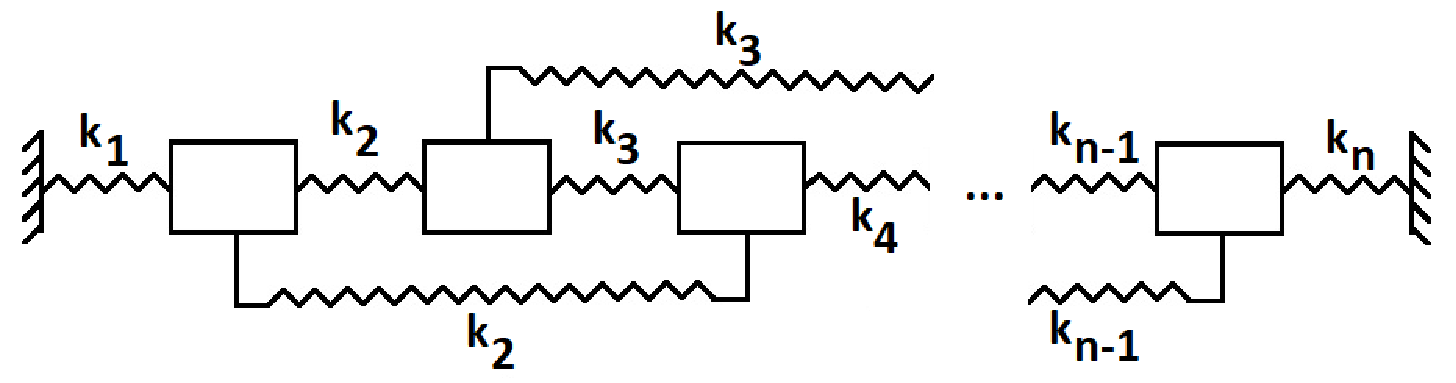
\includegraphics[width={3.0in}]{../figs/MassSys.pdf}
\centering
\caption{Equivalent spring/mass system used to generate the eigenvectors}
\label{fig:stiff}
\end{figure}

Note that the values chosen do not need to represent physical systems (e.g. negative stiffness values are acceptable).  
Other coupling systems were evaluated.  
However the best results corresponding to the system show in Fig.~\ref{fig:stiff}.  

Then, an eigenvalue problem is solved resulting in $n$ orthonormal eigenvectors used to represent the geometry for initial position $\theta=0$ (and all initial $phi$ positions).  
As the first vector tends to be planar motion (aka a cyclical vector) it is not chosen.  
This elimination results in a matrix formed by eigenvectors $2...m+1$.  
However, observations led to the conclusion that the orthogonal linear independence for $\theta=0$ caused some high $M$ values when considering all initial $\theta$ positions.  
Introducing linear dependence to the $\theta=0$ matrix was seen to result in decreased $M$ values for $\theta\neq 0$ combinations.  
To introduce linear dependence, a modified Gram-Schmidt orthogonality approach is used.  Specifically, 

\begin{equation}
\mathbf{E}^{new}_{d}=\mathbf{E}_{d}- c \sum_{e=1,...,n-1} \frac{\mathbf{E}_{e,e}^T \mathbf{E}_{d}}{\mathbf{E}_{e,e}^T \mathbf{E}_{e,e}}\mathbf{E}_{e,e},
\label{eq:GS}
\end{equation}

where $d$ denotes the $d^{th}$ eigenvector, $c$ is a constant between 0 and 1 such that 0 adds no linear dependence and 1 adds a portion of all other $\mathbf{E}_{e,e}$ vectors, and $e=1...n-1$ is the $e^{th}$ left shift of eigenvector $\mathbf{E}_e$. 
Thus, the similar component of shifted versions of each other vector, $\mathbf{E}_{e,e}$, is subtracted from the basis ($\theta=0$) vectors. 

This formulation leads to a decrease in the $M$ values, but an increase in the individual MAC values for the basis vectors as the non-shifted vectors are no longer orthogonal.
Other combinations of eigenvectors and shifts for $\mathbf{E}_{e,e}$ are acceptable, however a shift is required due to the initial orthogonality (otherwise there is no similar portion to subtract).

Next, the average of each new eigenvector is subtracted from the corresponding vector. 
Since mask material may only be added, the minimum value (plus the 0.1 cm addition to the geometry) is added to the eigenvector to make all the thicknesses positive.  
Lastly, each eigenvector is normalized by the maximum vector value and scaled. 
These steps produce a minimal thickness of approximately 0.1 cm and a maximum mask thickness of 7.87 inches.

Multiple geometries for various $k$ and $c$ combinations can be tested resulting in a design surface shown in Fig.~\ref{fig:surf}.  
These results are is based solely on the geometry vectors and not $\mathbf{DRM}_{red}$.  
Using this information, the settings with the lowest $M$ value can be chosen for the more time expensive MCNP simulations.

\begin{figure}[ht!]
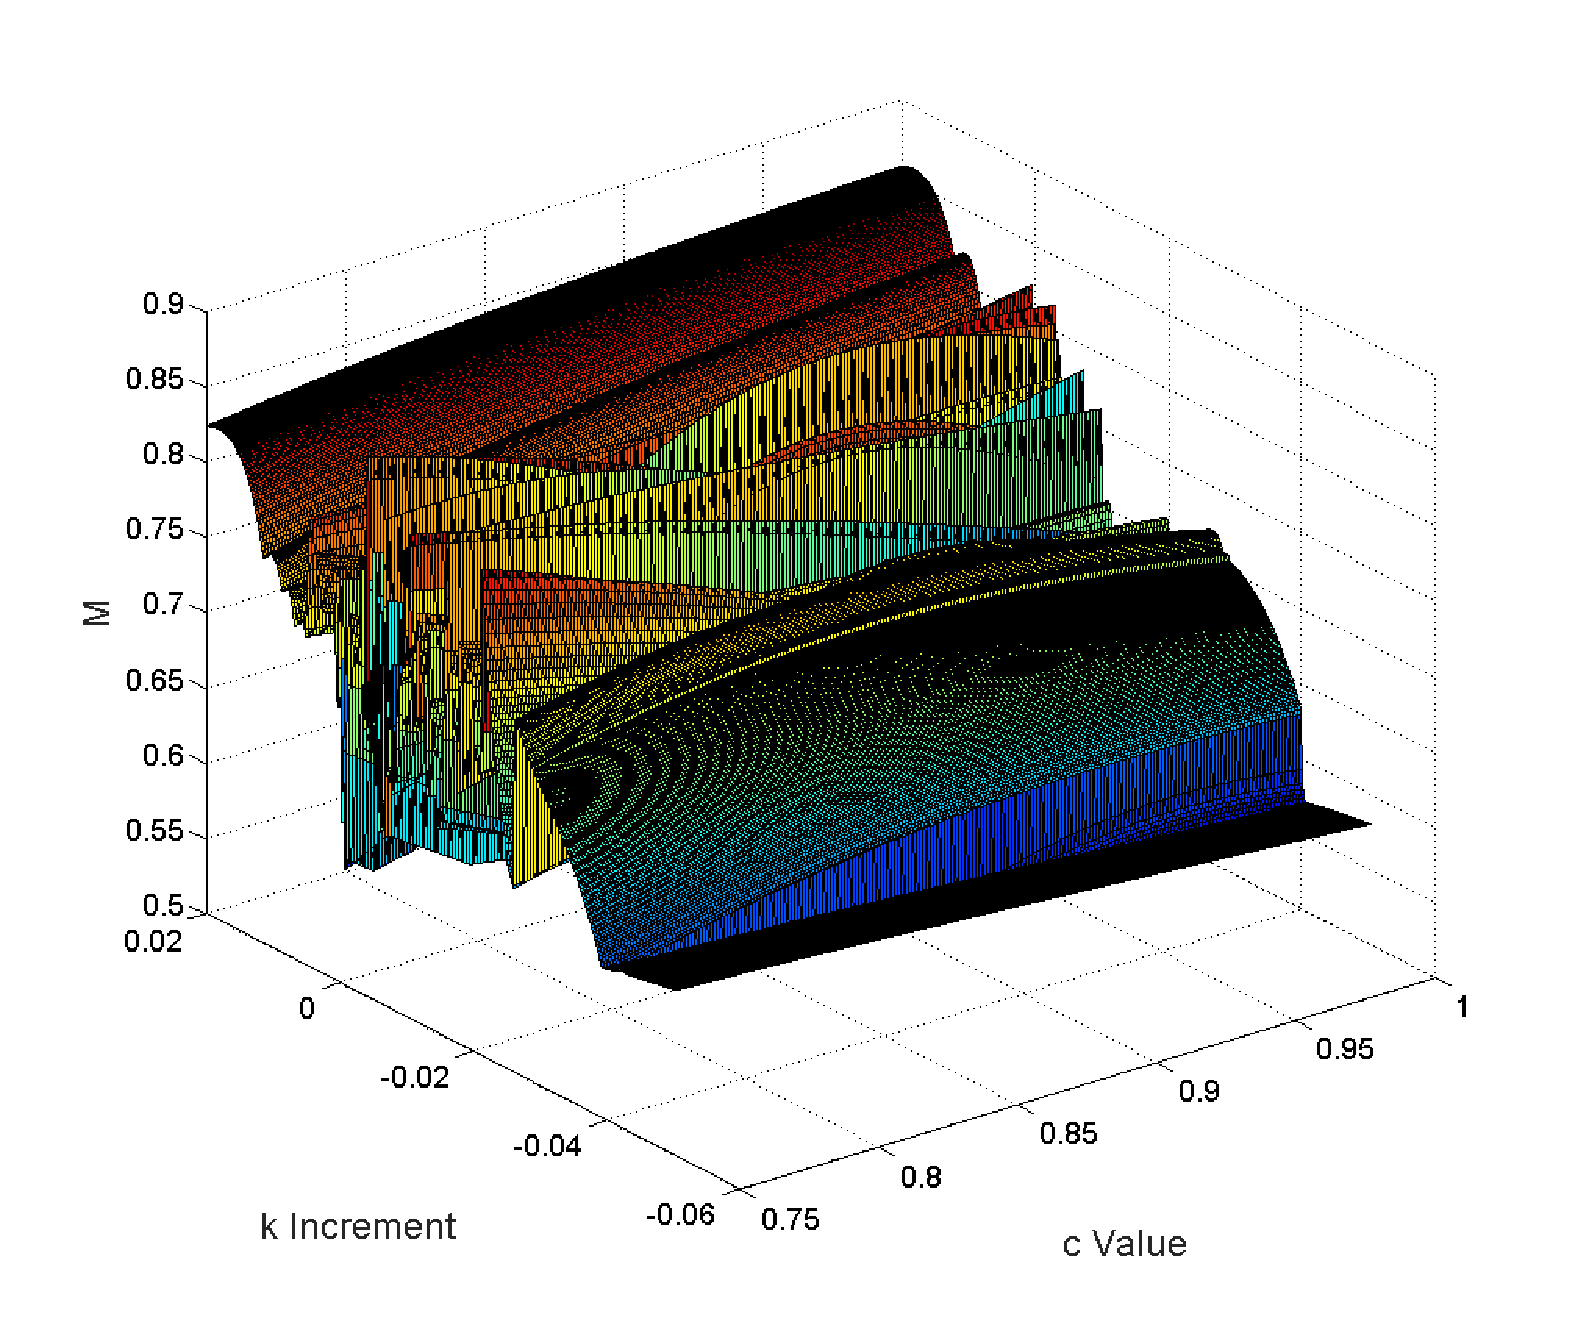
\includegraphics[width={3.0in}]{../figs/Eigprob32bitCouple2W1.pdf}
\centering
\caption{Surface generated by different $k$ step increments and $c$ values}
\label{fig:surf}
\end{figure}

\subsection{Binary Approach}
The binary approach uses ones and zeros to represent the geometry thickness.  
Notice that the mask's cyclic nature causes vectors such as [1 1 0 0] to be the same as [1 0 0 1] where the first vector is the second shifted by one entry to the right.  
If the design uses binary pattern such as these two, the DRCs for two initial positions will be identical.  
It can be proven for $n>7$ the best solution is to have any combination of vectors with three ones placed in an arrangement that avoids cyclic behavior with themselves (such as [1 0 1 0 1 0]) or others (such as [1 1 1 0 0 0] and 
[0 1 1 1 0 0]).  
The one exception is the inclusion of the binary "1" vector represented using 6 bits as [0 0 0 0 0 1]).  
These requirements yield the minimum possible $M$ value of 4/9 for any combination of binary geometry.  
For $n=32$, there are many possible basis vectors; especially considering that the vectors can be shifted left or right (corresponding to multiplication or division by 2) and the $\phi$ vector order (1st, 2nd, 3rd, etc) may be swapped.  
This flexibility allows one to create unique geometries, mechanically balance the mask, or improve the likelihood of obtaining a signal given a random source position by more evenly spreading the ones and zeros around the mask.

\subsection{Decoupling $\theta$ and $\phi$}
An alternative approach introduces additional material to create a low measurement "dead" zone at a consistent $\theta$ position.  
As a result, the initial $\theta$ position is assumed to be the angular distance difference between the start of the measurement and the minimum measurement location.  
The sign of the angle depends on the mask's rotation direction.  
It is conjectured that this association will be valid except when there are multiple sources in which spectral stripping is not possible  or for distributed sources.  
Further work in this area is ongoing.

As the initial $\theta$ position is known, by shifting the basis matrix entries by the corresponding index number the reference DRM angle may be changed to the known $\theta$ position.  
This knowledge decouples the $\theta$ and $\phi$ identification, resulting in only  needing to compare the measured DRC to the $m$ curves in $\mathbf{DRM}_{red}$.  
In this method, it is possible to create $m$ linearly independent geometric basis vectors.

One such linearly independent basis is the Hadamard matrix.  
While this matrix has been used in spectroscopy for many years, Hadamard encoding masks assume that some of cells are ``on", ``off" or detected by a second sensor\cite{DeVerse00}.  
In addition, it is assumed that one knows the on/off state of the cells.  
The equivalent RSM design goal is to identify this on/off state and thus, it corresponds to an inverse problem.  
In contracst to the encoding masks, each cell in the RSM design is not in a fully on/off state, but may have particles passing through it even when the source is not directly aligned.

The Hadamard matrix is thought to only exist for square matrices where $n$ is 1,2, or divisible by 4\cite{Sloane76}.  
By construction, the mask design under consideration is discretized in order to have $n=32$.  
Also, a Hadamard matrix has ones and negative ones.  
To convert it to a binary pattern, the negative one entries were changed to zeros.
In order to create the "dead" zone, the vector of ones corresponding to $\theta=0$ were changed to twos.  
A normalized geometry resulted by following the same steps as outlined in the eigenvector approach.

\section{Design Evaluation}
The maximum ($M$) and average ($A$) MAC numbers provide a method to evaluate the DRM's uniqueness.  
In addition, two other criteria provide information about a design's efficiency and sensitivity.
Note that the average, minimum, and maximum responses remains the same for different initial $\theta$ values.  
Thus, no $\theta$ shifting needs to be considered in the following formulations.  
A design that causes the detector to capture more particles results in more accurate results in less measurement time.  
Thus, the average number of particles for a cell for a given number
of source particles is in Eqn.~\ref{eq:avgcell}.  
This metric is related to the design's efficiency.

\begin{equation}
C=\frac{\sum_{i,j}\mathbf{DRM}_{red}}{n\ m}
\label{eq:avgcell}
\end{equation}
The final evaluation criterion focuses on the design's sensitivity.  The ratio of the maximum to minimum response in Eqn.~\ref{eq:sens} provides information on the relative amount of measurement time required and the measurement's sensitivity to random measurement noise. 
\begin{equation}
S=min_{j}\left(\frac{max_{i} \left[\mathbf{DRM}_{red}\right]}{min_{i} \left[\mathbf{DRM}_{red}\right]}\right)
\label{eq:sens}
\end{equation}

The following section applies these four evaluation criteria to DRC simulations for all possible discrete source positions.

\section{Results and Analysis}
The proposed design methodologies produced the geometries shown in Figs.~\ref{fig:EVGeo} to \ref{fig:HadGeo}.

\begin{figure}[ht!]
\centering
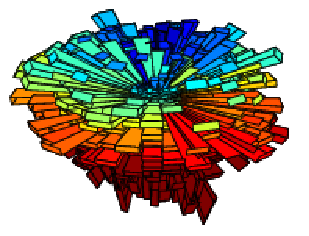
\includegraphics[width={2.0in}]{../figs/EVGeo.pdf}
\caption{RSM geometry created by the eigenvector approach}
\label{fig:EVGeo}
\end{figure}

\begin{figure}[ht!]
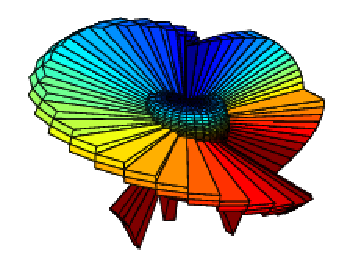
\includegraphics[width={2.0in}]{../figs/BiGeo.pdf}
\centering
\caption{RSM geometry created by the binary approach}
\label{fig:BiGeo}

The binary pattern was constructed to have a fin that spirals around the mask.  
As it is not possible to have the fin completely cover the mask geometry, four other vectors were added to created the needed basis.

\end{figure}
\begin{figure}[ht!]
\centering
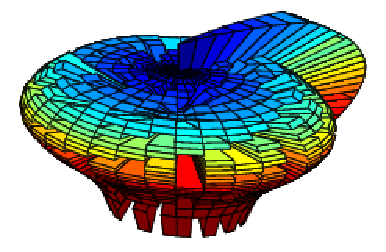
\includegraphics[width={2.0in}]{../figs/HadGeo.pdf}
\caption{RSM geometry created by the Hadamard approach}
\label{fig:HadGeo}
\end{figure}

The eigenvector approach used 32 $k$ values from 0.1 to -0.2999 in increments of -0.0129. c was 0.999.  
Other coupled systems did not have an optimal $c$ value close to one.

In order to establish whether a design is an improvement, first it is necessary to establish a baseline for comparison.  
Thus, FitzGerald's RSM's performance evaluation follows.  
Note that the simulation of FitzGerald's design involved a mask discretization of 10$^\circ$ in $\theta$ and $\phi$; corresponding to $n=36$.  
However, the Hadamard $n=36$ matrix cannot be created by lower order Hadamard matrices\cite{Weisstein}.  
Thus $n=32$ was used for the proposed designs instead.

Figure~\ref{fig:RSMMAC} shows a visual MAC number representation for $\theta=0$ obtained by using Eqn.~\ref{eq:mac}. 
 
\begin{figure}[ht!]
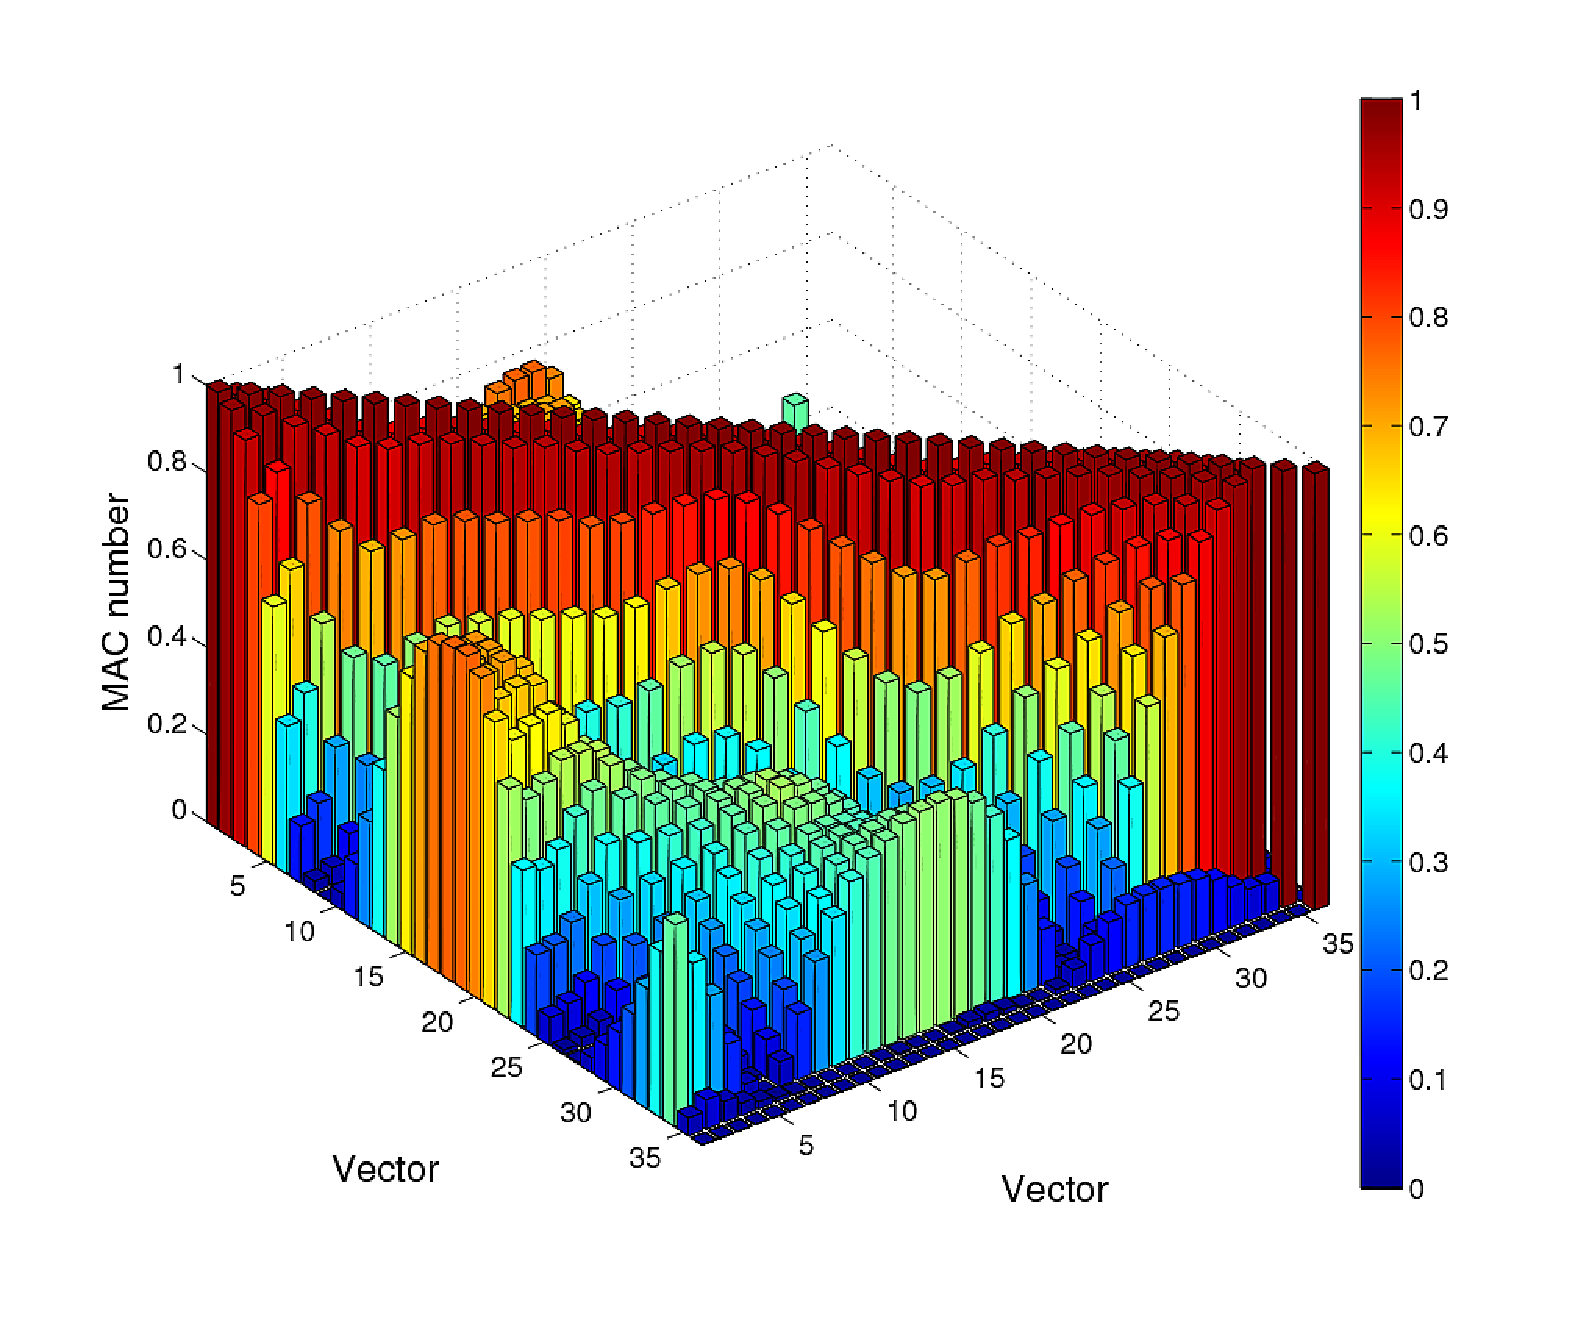
\includegraphics[width={3.0in}]{../figs/RSMMAC.pdf}
\centering
\caption{Representation of the original RSM MAC numbers for $\theta=0$}
\label{fig:RSMMAC}
\end{figure}

Note that the diagonal entries correspond to comparing a vector to itself, and thus will always be equal to one.  
The large off diagonal regions are of particular interest.  
These high values could result in the misidentification of the initial source position. 
In contrast, one may see the lower off-diagonal values resulting from the binary and eigenvector approaches in Figs.~\ref{fig:EMAC} to \ref{fig:HadMAC}.

\begin{figure}[ht!]
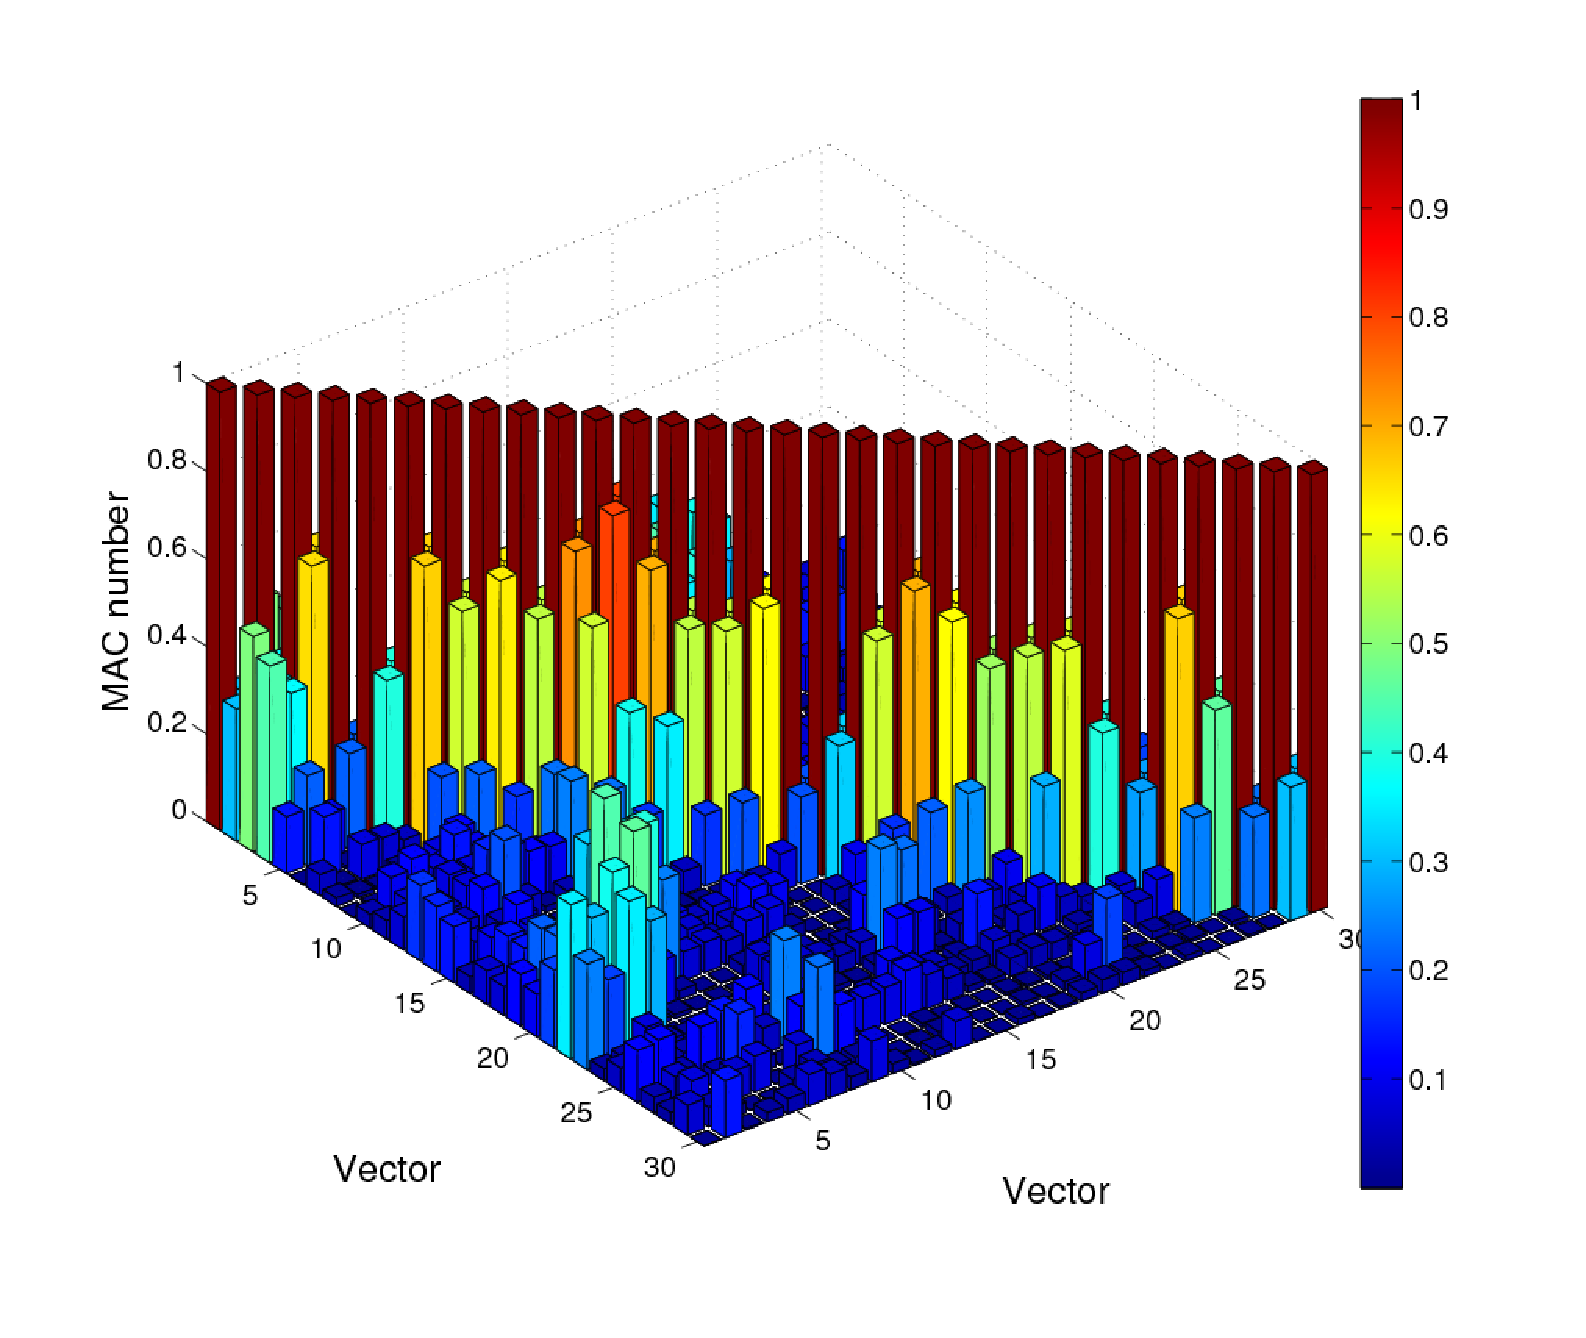
\includegraphics[width={3.0in}]{../figs/EVMAC.pdf}
\centering
\caption{Representation of the eigenvector RSM MAC numbers for the basis $\theta=0$}
\label{fig:EMAC}
\end{figure}

\begin{figure}[ht!]
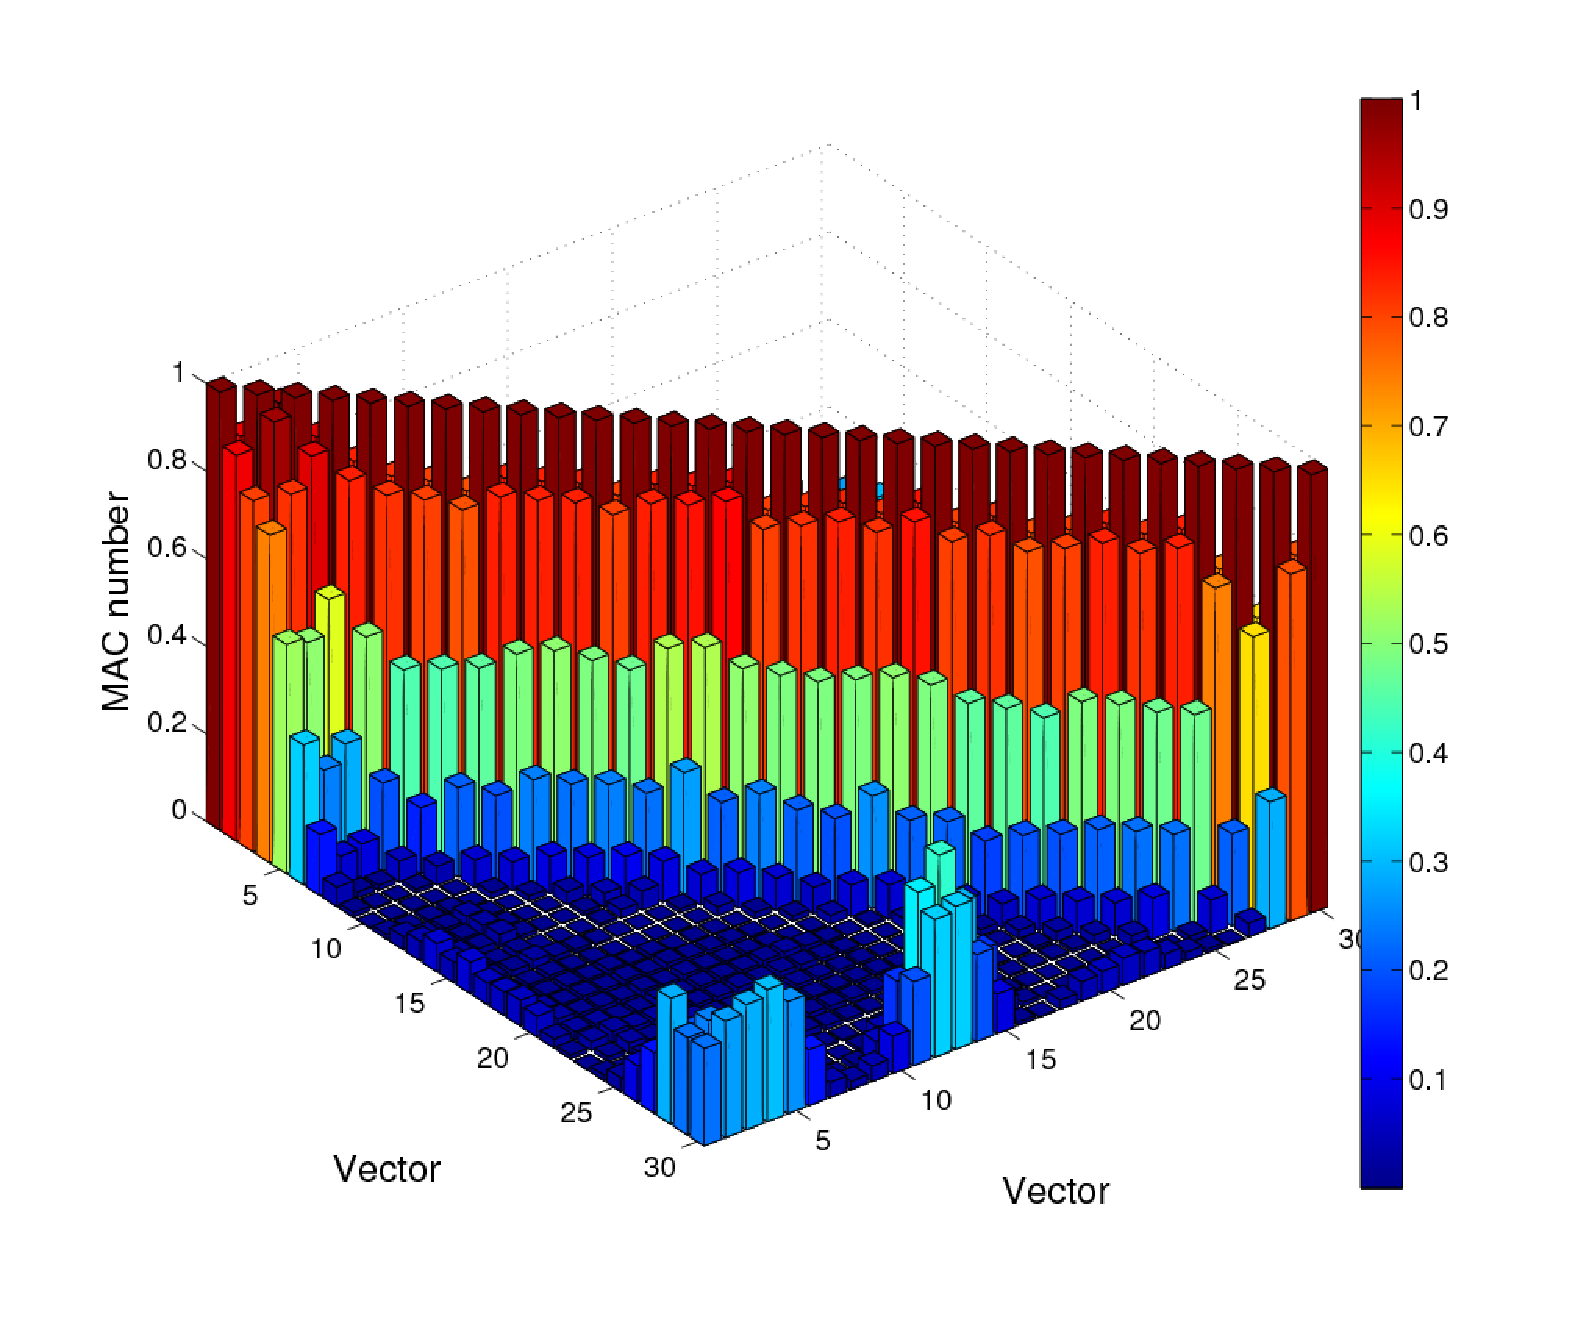
\includegraphics[width={3.0in}]{../figs/BiMAC.pdf}
\centering
\caption{Representation of the binary RSM MAC numbers for the basis $\theta=0$}
\label{fig:BMAC}
\end{figure}

\begin{figure}[ht!]
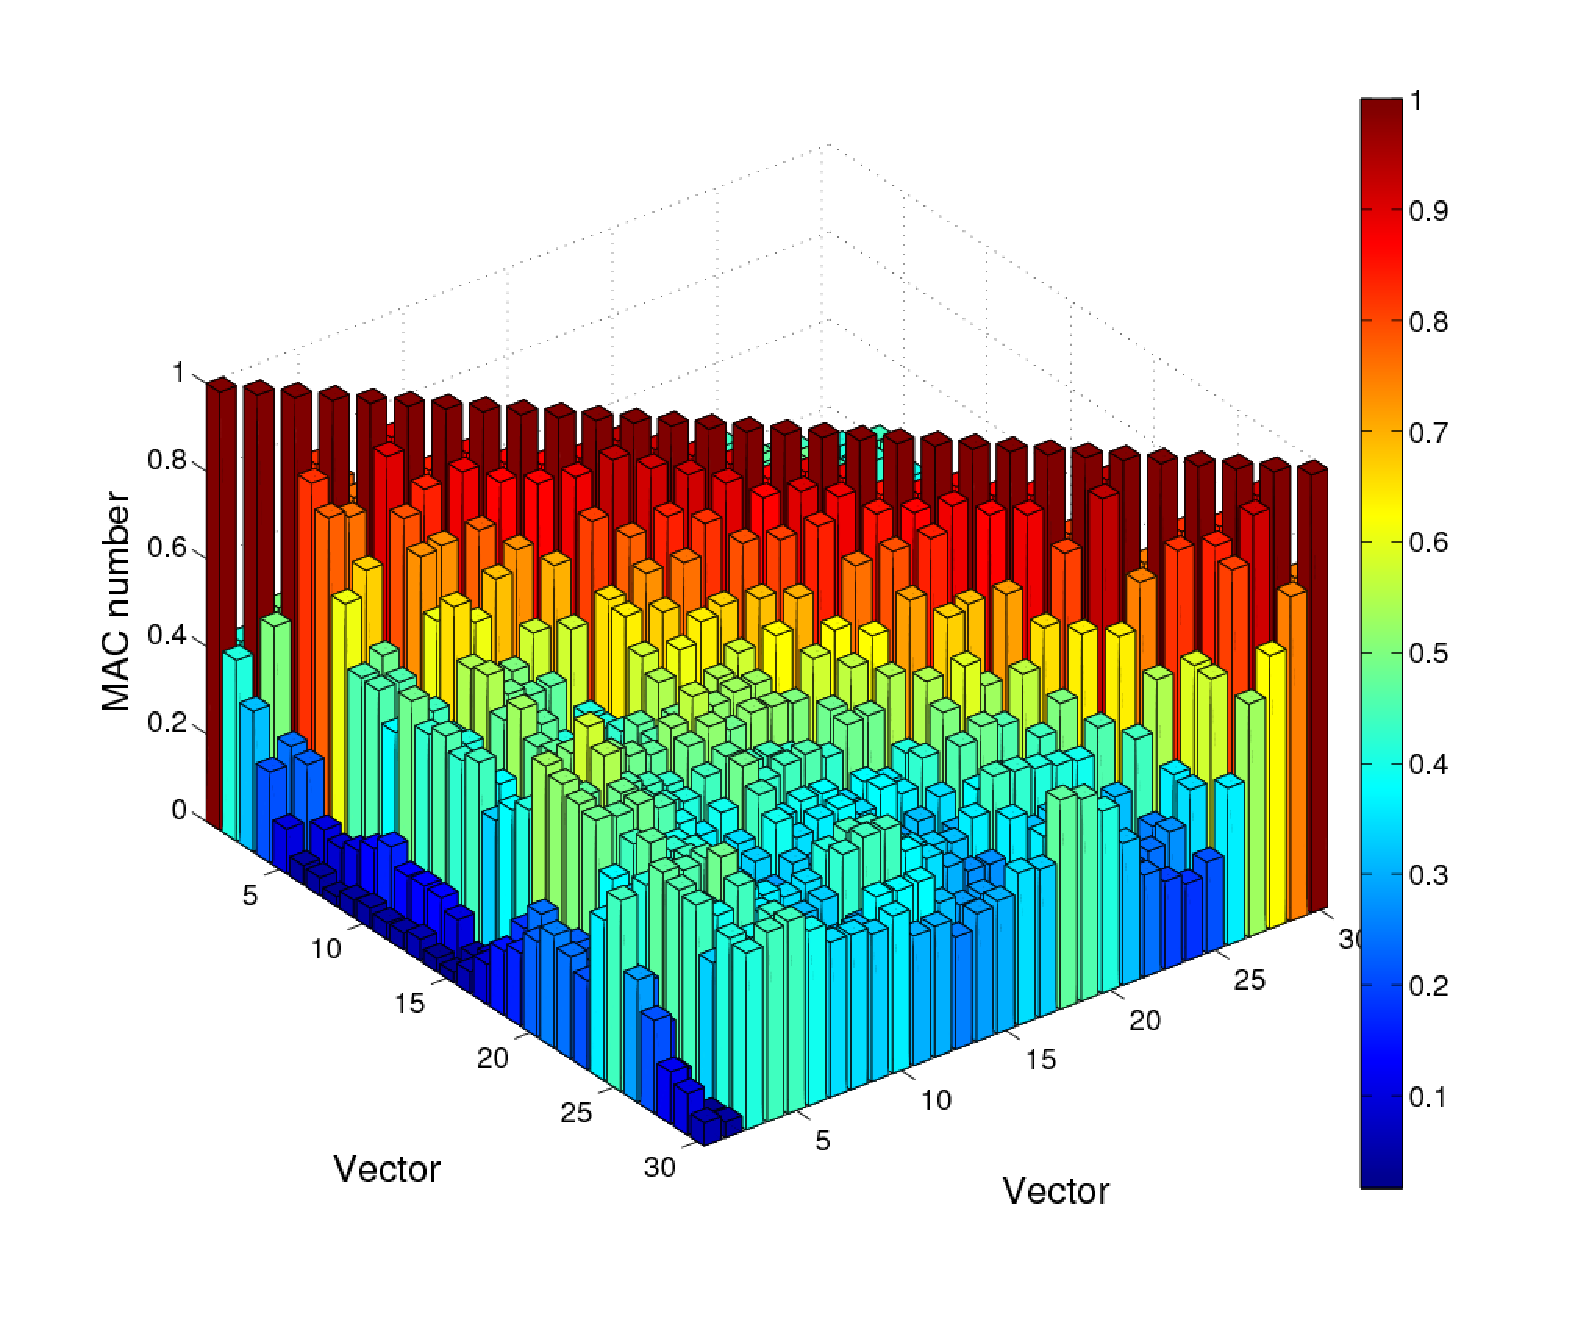
\includegraphics[width={3.0in}]{../figs/HadMAC.pdf}
\centering
\caption{Representation of the Hadamard MAC numbers for the basis $\theta=0$}
\label{fig:HadMAC}
\end{figure}

Note that the binary design may be improved by replacing the last four vectors with alternatives.  
The adjacent off-diagonal terms in Figs.~\ref{fig:RSMMAC}, \ref{fig:BMAC}, and ~\ref{fig:HadMAC} show that there is a limit to the spacial resolution.  
Specifically, for vector $p$, vectors $p+1$, $p+2$, and $p+3$ have MAC numbers that incrementally decrease.  
This behavior indicates that information is shared by neighboring initial positions.  
In the presence of measurement noise, it may only be possible to identity the position to an accuracy that is a multiple of the $\theta$ or $\phi$ discretization.

Table~\ref{table:results} summarizes the evaluation results for the original RSM, binary, eigenvector (EV), and Hadamard approaches.  
Recall that the Hadamard values correspond to those obtained without shifting vectors since the initial $\theta$ position can be deduced.

\begin{table}[ht]
\caption{Result Comparison from the Original and Proposed Designs} % title of Table
\centering % used for centering table
\begin{tabular}{|c|c|c|c|c|} % centered columns (4 columns)
\hline
Criteria & Original & EV & Binary & Hadamard\\
\hline
M & 1.00 & 0.808 & 0.963 & 0.935\\
\hline
A & 0.210 & 0.0663 & 0.125 & 0.423 \\
\hline
C $\left(\times 10^{-4}\right)$ & 3.75 & 2.96 & 3.86 & 3.70\\
\hline
S & 1.00 & 1.07 & 1.16 & 1.07 \\
\hline
\end{tabular}
\label{table:results} % is used to refer this table in the text
\end{table}

Notice that the original design has an overall MAC number of 1.00. 
This value corresponds to a part of the geometry that has a constant thickness as $\theta$ varies.  
As a result, a shift in the initial $\theta$ produces the same DRC and a MAC number of 1.  
For the same reason, the sensitivity value is 1.00.  
In contrast, the proposed methods have lower $M$ values with the most desirable corresponding to the eigenvector approach.  
The Hadamard method produces vectors which on average share 42.3\% of their information, which is more than the original design.  
The rapid change between ones and zeros coupled with the spacial resolution limits make the Hadamard method non-ideal for this problem.  
The lowest average MAC number corresponds to the eigenvector approach with only 6.63\% similarity.  
These results indicate that the method that produces the most unique
DRCs is the eigenvector approach.  
However, the trade-off is that the eigenvector method produced a RSM with a lower average normalized number of counts per cell.  
The binary method has the most average normalized number of counts per cell, but also the highest sensitivity.  
This high sensitivity may indicate that certain initial positions are more susceptible to measurement noise.

\section{Conclusions}
This work introduced three methods to optimize a rotating scatter mask's geometry for a gamma source location identification.  
The results indicate that the original RSM design has multiple source positions that produce the same or similar detector response curves.  
This issue may result in an incorrect source position identification.
The eigenvector approach produced more unique detector response curves than the original and other methodologies. 
Unfortunately there is a corresponding decrease in the average normalized counts per cell, thus this mask requires 21\% more particles and longer measurement times to produce the same measurement accuracy as the original design.

While these results demonstrate the binary and eigenvector methods decrease the overall and average linear dependence of the DRCs, more optimal designs may exist.  Specifically, choosing an alternative last four vectors for the binary pattern may reduce the corresponding off-diagonal MAC terms.  
As a result, $A$ should decrease.  
In addition, rotating or swapping the binary vectors would allow for a better mechanical balance.  
The eigenvector approach has a large design space especially when other coupled systems are considered.  
Further exploration of this space and its refinement may produce a geometry with lower $M$ and $A$ values.

\section{Acknowledgment}
This work was supported though the Air Force Summer Faculty Program and the Air Force Institute of Technology.  
The author would to thank Dr. Larry Burggraf and Dr. Adam Cahill for their assistance and insightful input to this work.

\appendix

\section{Proof}
%% The Appendices part is started with the command \appendix;
%% appendix sections are then done as normal sections
%% \appendix

%% \section{}
%% \label{}
Goal: Choose $n$ binary numbers such that the MAC number denoted as 

\begin{equation}
MAC_{a,b}=\frac{\left(\mathbf{a}\cdot\mathbf{b}\right)^2}{\left(\mathbf{a}\cdot\mathbf{a}\right)\left(\mathbf{b}\cdot\mathbf{b}\right)}
\end{equation}

is minimized for every combination of numbers $a$ and $b$ including their the corresponding cyclically shifted versions.

Consider an $n$ bit binary number greater than zero with $p$ ones and $n-p$ zeros, where $0<p<n$.  
Further, shift this number by any number of bits so that the left-most bit contains a one.  
Because of the cyclic nature, the binary number can be written as a vector containing the integer number of zeros bounded on either end by ones.  
For example, the number 0 1 1 would be shifted to 1 0 1 and could be written as the vector [1].  
Also, the number [0 1 0 1 0 1 0 0] can be shifted to [1 0 1 0 1 0 0 0], and the corresponding vector is [1 1 3].  
Recall that the vector's cyclic nature causes the last one to wrap around to the first 
position.  
In general, we can write any non-zero binary number as the vector $\textbf{v}=\left[v_1\ v_2\ v_3\ \cdots\ v_p\right]$, where each $v_i$ is the number of zeros between two ones and $v_p=n-p-\sum\limits_{i} v_i$.  

Now, cyclic redundancy can be avoided by ignoring any $\textbf{v}$ that become duplicated under shifts.  
For example, [0 3 2] and [3 2 0] represented the same binary number, where the second vector is the first shifted to the left by $v_1+2$ bits.  
To avoid this behavior, we require $v_{1}<v_p$, but $v_2\le v_p, v_3\le v_p, \cdots, v_{p-1}\le v_p$.  
Note that by construction two vectors with a different number of ones cannot be cyclically identical.

Consider two vectors, $\textbf{u}=\left[u_1\ u_2\ u_3\ \cdots\ u_{p_u}\right]$ and $\textbf{v}=\left[v_1\ v_2\ v_3\ \cdots\ v_{p_v}\right]$ containing $p_u$ and $p_v$ ones respectively.  
If $u_i=v_i$ the vector has at least two ones in the corresponding binary number that would align for some shift of $\textbf{u}$.  
We want to choose $n$ vectors, which $a_1, a_2, ... a_n$ that produce the minimum value of $max\left\{MAC_{a_1...a_n}\right\}$, where the maximum is taken over all possible shifts of $\textbf{a}_i, \textbf{a}_j$, $i=1...n$, and $j=1...n$.  
Note that if $i=j$, then the second vector must be shifted by at least one bit to avoid comparing a vector with itself.  
For a binary number undergoing all possible shifts, the denominator becomes $p_u * p_v$, while the numerator is the square of the total number of ones that simultaneously align as each vector is rotated.  
As the number of ones increases, both the numerator and denominator increase.   
Thus, it becomes unclear if the MAC number increases or decreases as $p_u$ and/or $p_v$ increase.

First, consider $p=1$.  
There is only one vector, which can be expressed as $\left[n-1\right]$.  
There are no other possible non-cyclically redundant combinations.  
Letting $a$ and $b$ be this vector results in a maximum MAC number of $\frac{0}{1*1}=0$.

Next, consider $p=2$.  
Possible vectors include $[0\ n-p], [1\  n-p-1], [2\ n-p-2], \cdots, [\frac{n-p-1}{2}\ \frac{n-p+1}{2}]$ if $n$ is odd or a limit of $[\frac{n-p}{2}-1\ \frac{n-p}{2}+1]$ if $n$ is even. 
Note that there are only $\frac{n-p+1}{2}$ if $n$ is odd and $\frac{n-p}{2}$ if $n$ is even possible vectors of type $p=2$, but $n$ are required.  
Thus, more vectors from other $p$ types would be required to complete the basis set.  
By construction, all of the indices are unique indicating that only one 1 aligns over all possible rotations (if two aligned, then the vectors would in fact be identical). 
Thus, the maximum MAC number, when using any two $p=2$ vectors is $\frac{1^2}{2*2}=1/4$.

Consider $p=3$.  
Let $m=\lfloor\frac{n-p-1}{p}\rfloor$, $q=\lfloor\frac{n-p}{2}\rfloor$, and $s$ is 0 if $n$ is odd and 1 if $n$ is even. 
The possible vectors are sets of decreasing size

\begin{center}
$\{[0,\ 0,\ n-p-0]; [0,\ 1,\ n-p-1]; \cdots [0,\ q-0,\ q+s-0]\}$,\\
$\{[1,\ 0,\ n-p-1]; [1,\ 1,\ n-p-2]; \cdots [1,\ q+s-1,\ q-0]\}$,\\
$\{[2,\ 0,\ n-p-2]; [2,\ 1,\ n-p-3]; \cdots [2,\ q-1,\ q+s-1]\}$,\\
$\{[3,\ 0,\ n-p-3]; [3,\ 1,\ n-p-4]; \cdots [3,\ q+s-2,\ q-1]\}$,\\
$\{[4,\ 0,\ n-p-4]; [4,\ 1,\ n-p-5]; \cdots [4,\ q-2,\ q+s-2]\}$,\\
$\vdots$ \\
$\{[m,\ 0,\ n-p-m], [m,\ 1,\ n-p-m-1], \cdots [m,\ q-\lfloor \frac{m+1}{2}\rfloor+s\ mod(m,2),\ q-\lfloor \frac{m}{2}\rfloor+s\ mod(m+1,2)]\}$,
\end{center}

In general, the $kth$ set can be expressed as 

\begin{equation}
\{[k,\ 0,\ n-p-k], [k,\ 1,\ n-p-k-1], \cdots [k,\ q-\lfloor \frac{k+1}{2}\rfloor+s\ mod(k,2),\ q-\lfloor \frac{k}{2}\rfloor+s\ mod(k+1,2)]\},
\end{equation}

where the total number of terms, $t_1$, is

\begin{equation}
t_1=\sum_{k=0}^{m} \lfloor\frac{n-p}{2}\rfloor-\lfloor\frac{k+1}{2}\rfloor+s\ mod(k,2)+1.
\end{equation}

Since $v_1<v_3$, sets with $v_1>m$, can be expressed using the following approach,

\begin{center}
$\{[m+1,\ 0,\ n-p-m-1]; [m+1,\ 1,\ n-p-m-2]; \cdots [m+1,\ n-p-2m-3,\ m+2]\}$,\\
$\{[m+2,\ 0,\ n-p-m-2]; [m+2,\ 1,\ n-p-m-3]; \cdots [m+2,\ n-p-2m-5,\ m+3]\}$,\\
$\{[m+3,\ 0,\ n-p-m-3]; [m+3,\ 1,\ n-p-m-4]; \cdots [m+3,\ n-p-2m-7,\ m+4]\}$,\\
$\vdots$ \\
\end{center}

\begin{center}
$\{[\lfloor\frac{n-p-1}{2}\rfloor,\ 0,\ q+1]\}$ if $n$ is even.\\
$\{[\lfloor\frac{n-p-1}{2}\rfloor,\ 0,\ q+1]; [\lfloor\frac{n-p-1}{2}\rfloor,\ 1,\ q]\}$ if $n$ is odd.
\end{center} 

In general, the $kth$ set can be expressed as 

\begin{equation}
\{[k,\ 0,\ n-p-k-0], [k,\ 1,\ n-p-k-1], \cdots [k,\ n-p-2k-1,\ k+1]\},
\end{equation}

where the total number of terms, $t_2$, is

\begin{equation}
t_2=\sum_{k=m+1}^{\lfloor\frac{n-p-1}{2}\rfloor} n-p-2k-1+1 =\sum_{k=m+1}^{\lfloor\frac{n-p-1}{2}\rfloor} n-p-2k
\end{equation}

Thus, the total number of terms for $n$ and $p=3$ is $t=t_1+t_2$.  

%Since the $v_p$ term is dependent on the $v_1 ... v_{p-1}$ terms, the number of possible repeated terms is $p-1$.  Thus, if $r>p-1$, it is not possible to form a complete basis from just this one p-type. 
Let the matrix $\textbf{V}$ contain terms $V_{ij}=v_i$ for the $jth$ basis vector including the dependent $v_p$, where $1<i<p$ and $1<j<n$.

For a given $n$ and $p$, the number of unique indices is less than or equal to $\lfloor \frac{n-p}{2}\rfloor+1$ since $v_i\le v_p$.  
To form an $n$ vector basis requires $n\left(p-1\right)$ total entries.  
Thus, it is not possible for any column in $\textbf{V}$ to contain only unique indices since $n>\lfloor \frac{n-p}{2}\rfloor+1$ and $r\ge 1$ for $p\ge2$.  
Also, it is impossible to from a complete basis for $p=2$.  
In addition, for $p=3$ the maximum MAC number is $\frac{2^2}{3*3}=4/9$, where one duplicate index results in two aligned 1s.

Note that the $p=1$ vector can be combined with the $p=3$ vectors, since the maximum MAC number between a $p=1$ and $p=3$ vector is $\frac{1^2}{1*3}=1/3 < 4/9$ (only one ``1" can align).  
Figure~\ref{fig:terms} shows that the number of possible terms (including $p=1$) equals ($n=8$) or exceeds $n$ ($8<n\le 360$).  
Due to manufacturing constraints, $n$ was limited to 360 as this corresponds to one degree increments in $\theta$ and 0.5 degree in $\phi$.  
As a result, a full basis can be formed from these vectors if $n>7$.

\begin{figure}[ht!]
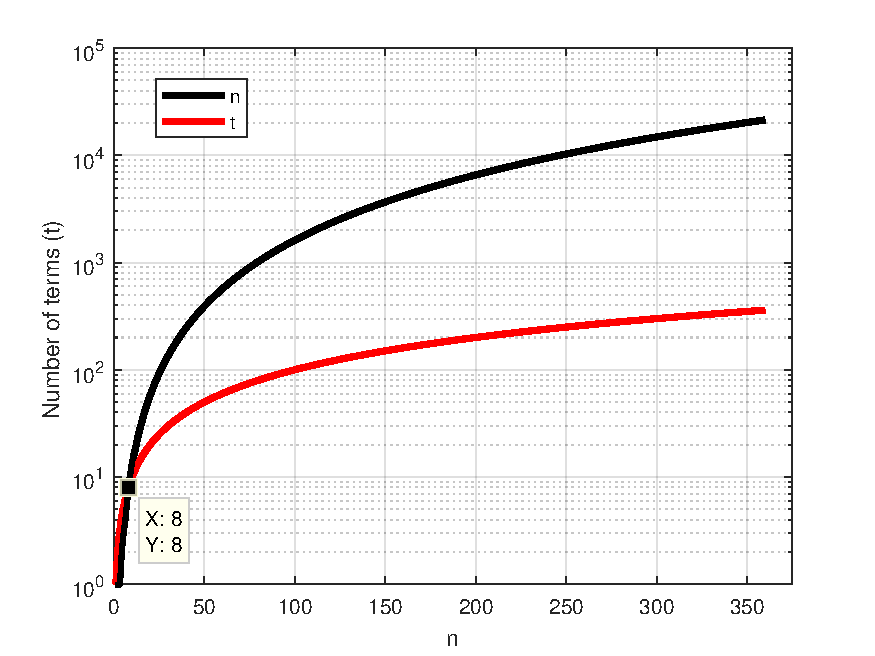
\includegraphics[width={3.0in}]{../figs/TermPlot.pdf}
\centering
\caption{The number of possible terms for $p=1$ and 3 equals or exceeds $n$ if $n>7$.}
\label{fig:terms}
\end{figure}

Now, consider creating a $p>3$ basis.  
Let $r$ represent the greatest number of repeated indices for any two basis vectors.
Note that the minimum number of aligned 1s is $r+1$
The maximum MAC number can then be expressed as

\begin{equation}
MAC_{a,b}\ge\frac{\left(r+1\right)^2}{p_a p_b},
\end{equation}
where $p_a$ and $p_b$ are the p-type of vectors $a$ and $p$ respectively.  If one chooses vectors from the same p-type, then $p_a=p_b=p$ and
\begin{equation}
MAC_{a,b}\ge\frac{\left(r+1\right)^2}{p^2},
\end{equation}

%Consider two columns in $\textbf{V}$ corresponding to $p\ge3$.  For $r$ to not increase, $V_{1j}$ and $V_{2j}$ must be drawn from the $\lfloor \frac{n-p}{2}\rfloor+1$ indices such that $V_{1j}+V_{2j}\le n-p$.  Possible combinations include $0\ 0, 0\ 1,\ ...\ 0\ \lfloor \frac{n-p}{2}\rfloor+1, 1\ 0, 1\ 1,\ ...\ 1 \lfloor \frac{n-p}{2}\rfloor,\ ...\ \lfloor \frac{n-p}{2}\rfloor+1\ 0$. The total is 
%\begin{equation}
%\sum_{k=1}^{\lfloor \frac{n-p}{2}\rfloor+2} k = \frac{\left(\lfloor \frac{n-p}{2}\rfloor+2\right) \left(\lfloor \frac{n-p}{2}\rfloor+3\right)}{2}
%\end{equation}
%Note that as $p$ increases, there are fewer possibilities.  To avoid $r=2$, there must be at least $2n$ possibilities.

%% References
%%
%% Following citation commands can be used in the body text:
%% Usage of \cite is as follows:
%%   \cite{key}         ==>>  [#]
%%   \cite[chap. 2]{key} ==>> [#, chap. 2]
%%

%% References with BibTeX database:

\bibliographystyle{elsarticle-num}
\bibliography{RSM}

%% Authors are advised to use a BibTeX database file for their reference list.
%% The provided style file elsarticle-num.bst formats references in the required Procedia style

%% For references without a BibTeX database:

% \begin{thebibliography}{00}

%% \bibitem must have the following form:
%%   \bibitem{key}...
%%

% \bibitem{}

% \end{thebibliography}

\end{document}

%%
%% End of file `ecrc-template.tex'. 